\chapter{Firebase}

Das nächste Kapitel beschreibt die Architektur und die Implementierung der geplanten Anwendung mit Google Firebase.

\section{Architektur}

Für die Architektur wird zunächst die Lösungsstrategie vorgestellt. Darauf folgen die Bausteinsicht, die Laufzeitsicht sowie die Verteilungssicht.

\subsection{Lösungsstrategie}

Ebenfalls wie bei \ac{AWS} Amplify lässt sich die Architektur von Firebase in Präsentation, Logik und Datenhaltung aufteilen, welche durch unterschiedliche Cloud-Dienste und Frameworks abgebildet sind.
\begin{itemize}
  \item Präsentation
    \begin{itemize}
      \item React.js mit TypeScript
      \item Firebase Javascript SDK
    \end{itemize}
  \item Logik
    \begin{itemize}
      \item Authentication
      \item Cloud Functions
      \item Transcoder API
    \end{itemize}
  \item Datenhaltung
    \begin{itemize}
      \item Authentication
      \item Cloud Firestore
      \item Cloud Storage
      \item IAM
      \item Firebase Hosting
    \end{itemize}
\end{itemize}

Auch hier werden ausschließlich interne Dienste der Google Cloud verwendet, so dass die Rahmenbedingungen nicht missachtet sind und die beiden Technologien vergleichbar sind. Abgesehen von Cloud-Diensten ist der Unterschied beider Projekte auf technischer Ebene, dass die Firebase-Anwendung im Backend TypeScript statt JavaScript verwendet.

Als nächstes werden Lösungsansätze, um die nichtfunktionalen Anforderungen, auch Qualitätsziele genannt, zu erreichen:

\begin{description}
   \item[Verfügbarkeit] Firebase bietet für Frontend und Backend ein Zero-Downtime Deployment.
   \item[Skalierbarkeit] Durch die Serverless-Architektur skalieren Funktionen sowie Firestore automatisch innerhalb der Google-Cloud.
   \item[Analysierbarkeit] Durch den Einsatz von Cloud Logging können Anfragen für Funktionen nachvollzogen werden.
   \item[Interoperabilität] Es wird keine REST- oder GraphQL-Schnittstelle genutzt. Stattdessen werden die Funktionen des Backends direkt aufgerufen. Damit ist die Interoperabilität nicht direkt gegeben.
   \item[Backups] Backups lassen sich automatisiert über Firestore aktivieren.
   \item[Wiederherstellbarkeit] Das Backup von Firestore muss manuell eingespielt werden.
\end{description}

\subsection{Bausteinsicht}

Wie bei \ac{AWS} Amplify gibt es eine Unterteilung zwischen Frontend, auf das dieses Kapitel nicht näher eingeht und dem Backend, welches wichtig für die Vergleichbarkeit der Anwendungen ist. Das Backend besteht aus den folgenden Bausteinen:

\begin{itemize}
  \item{Der Dienst \textit{Authentication} regelt die Authentifizierung und die Autorisierung von Benutzern.}
  \item{Der Dienst \textit{Cloud Functions} stellt die folgenden Funktionen zur Verfügung, die in Form einer Schnittstelle an das Frontend freigegeben werden:}
  \begin{itemize}
    \item CreateVideo
    \item AddWatermark
    \item UpdateVideo
    \item DeleteVideo
    \item GetVideo
  \end{itemize}
  \item{Die \textit{Transcoder API} stellt eine Schnittstelle zur Verfügung, um Videos mit Wasserzeichen zu versehen und abzuspeichern.}
  \item{Die Datenbank \textit{Cloud Firestore} speichert alle Videos sowie eine Liste aller Administratoren der Anwendung ab.}
  \item{Das Dateisystem \textit{Cloud Storage} speichert alle Video-Dateien ab.}
\end{itemize}

\subsection{Laufzeitsicht}

Die Laufzeitsicht beschreibt die wichtigsten Prozesse und wie die Bausteine miteinander interagieren.

\subsubsection{Auflisten, Aktualisieren und Löschen eines Videos}

\begin{figure}
  \centering
  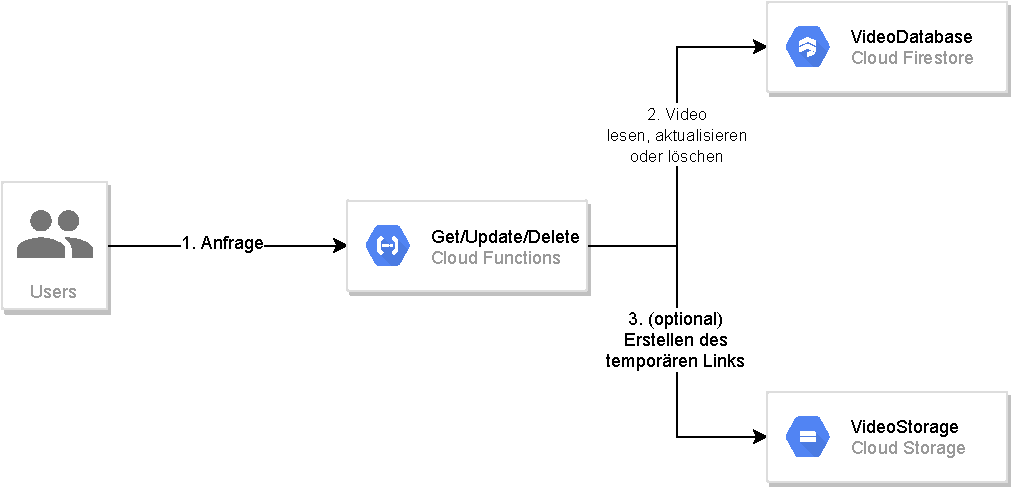
\includegraphics[width=1\columnwidth]{6_firebase/laufzeitsicht_1.pdf}
  \caption{Firebase - Laufzeitsicht - Auflisten, Aktualisieren und Löschen eines Videos}
  \label{Firebase:laufzeitsicht1}
\end{figure}

\autoref{Firebase:laufzeitsicht1} stellt den Prozess, wie Videos von Nutzern aufgelistet, aktualisiert oder gelöscht werden, dar. Dieser wird im folgenden Abschnitt näher erläutert:

\begin{enumerate}
  \item{Der Nutzer stellt eine Anfrage mittels eines Funktionsaufrufs, der den JSON Webtoken und weitere Funktionsparameter mitsendet.}
  \item{Der Nutzer wird autorisiert und die Funktion wird mit einer Kontext-Variable, die den Nutzer enthält, ausgeführt. Die Funktion führt nun weitere Anfragen an Firestore und optional an Storage aus.}
  \item{Die Rechteprüfungen beim Aktualisieren oder Löschen des Videos werden selbst durchgeführt, indem eine Liste aller Administratoren geholt wird.}
  \item{Handelt es sich um eine Anfrage zum Auflisten, werden aus der Video-Tabelle alle Datensätze unter Berücksichtigung des Suchfelds geholt. Bei den Abfragen zum Aktualisieren oder zum Löschen prüft die Funktion das Besitzer-Attribut, sofern der Nutzer kein Administrator ist.}
  \item{Handelt es sich um eine Anfrage zum Auflisten, werden signierte temporäre Links über den Service Storage erstellt.}
\end{enumerate}

\subsubsection{Erstellen eines Videos}

\begin{figure}
  \centering
  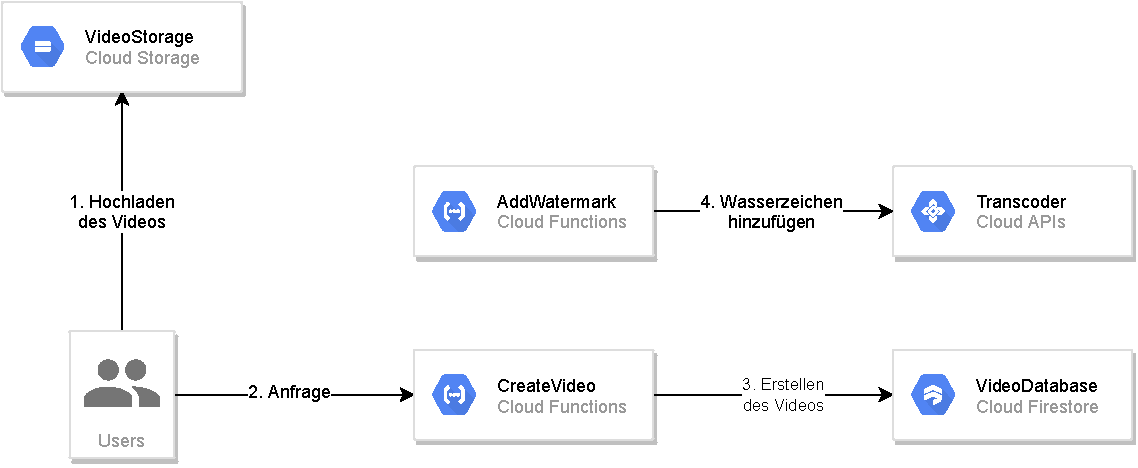
\includegraphics[width=1\columnwidth]{6_firebase/laufzeitsicht_2.pdf}
  \caption{Firebase - Laufzeitsicht - Erstellen eines Videos}
  \label{Firebase:laufzeitsicht2}
\end{figure}

\autoref{Firebase:laufzeitsicht2} stellt den Prozess des Erstellens eines Videos dar.
\begin{enumerate}
  \item{Zu Beginn lädt der Nutzer das Video in einen gemeinsamen Ordner im Storage hoch. Der Storage ist nach außen hin nicht aufrufbar.}
  \item{Dann ruft der Nutzer die Funktion im Backend auf und gibt den JSON Webtoken sowie die weiteren Parameter wie die URL des Videos im Storage, den Titel und die Beschreibung des Videos mit.}
  \item{Die entsprechende Funktion wird ausgeführt, welche die Informationen in Firestore abspeichert.}
  \item{Aufgrund des neuen Eintrags in Firestore, wird die Wasserzeichen-Funktion ausgelöst. Diese stellt eine Anfrage an die Transcoder-API und speichert den neuen Link zum verarbeiteten Video wieder im Storage.}
\end{enumerate}

\subsection{Verteilungssicht}

\begin{figure}
  \centering
  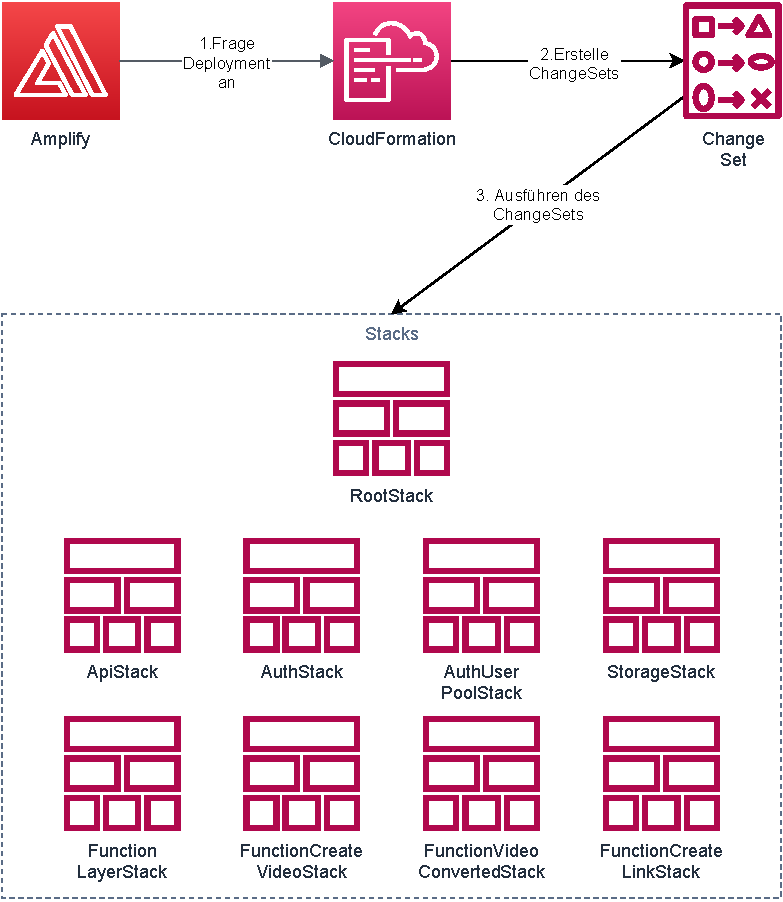
\includegraphics[width=0.75\columnwidth]{6_firebase/verteilungssicht.pdf}
  \caption{Firebase - Verteilungssicht}
  \label{Firebase:verteilungssicht}
\end{figure}

\autoref{Firebase:verteilungssicht} stellt dar, wie die Anwendung bereitgestellt wird.

Im Gegensatz zu \ac{AWS} Amplify verwendet Firebase keine Stacks, sondern stellt die einzelnen Dienste über eine REST-API zur Verfügung. Diese lässt sich über das Command-Line Interface aufrufen. Alternativ kann die Schnittstelle auch direkt angesprochen werden. Die Anwendung benötigt diese Funktionalität allerdings nicht, da keine speziellen Anforderungen an das Deployment bestehen und damit der Standard ausreicht.

\section{Implementierung}

todo